\label{ch:4}
\begin{comment}
\textcolor{red!40!black}{
In this important chapter I want the explain how Majoranas are localized in defects and to calculate in mean-field approximation the phase diagram. 
\begin{itemize}
    \item Brief explanation of how linear defects may be formed in the \acrshort{rucl} by stacking faults; [Need to study more! also : look for numerical values for the coupling and dependence with the distance];
    \item Consider a local experiment near the defect as two adjacent Kitaev materials being proximate. The (homogeneous) coupling $\tilde{J}$ between the two material describe a (apparently second order) phase transition from a non-interacting to a hybridized one at finite critical coupling $\tilde{J}_c$. 
    \item Perform the calculation in mean-field approximation: set two homogeneous order parameter, Fourier transform in x-direction, perform a unitary transformation, %(analytically unknown,  but numerically know)
     calculate self-consistently (numerically) the order parameters, find the phase diagram ( $\tilde{J}_c$ as function of $h$);
\end{itemize}
As long as the defect is \say{wider enough}, so that the effective coupling $\tilde{J}$ is smaller than $\tilde{J}_c$, it will harbors localized gapless chiral Majorana fermions.}
\pagebreak 
\end{comment}
%%%%%%%%%%%%%%%%%%%%%%%%%%%%%%%%%%%%%%%%%%%%%%%%%%%%%%%%%%%%%%%%%%%%%%%%%%%


The fundamentals for the Kitaev model were described in the previous chapters, and now I will start the description of the defects. This work does not intend to be a study of all types of defects in Kitaev material. %Actually, the much more humble goal of this work consists of study a particular type of defect.
%Majorana modes in the gapped (B) phase lives in the edge of the material. %The defects that I am interested are those whose mimics a edge, but inside the bulk. Even beside this types of defects, I will only study one simple case in which the defect happens in a straight line along the $a$ direction as shown in \ref{fig:4-defect}.
In this work I will focus on a particular the of one-dimensional defect characterized by broken bonds on a straight line along the $a$ direction as show in the figure \ref{fig:4-defect}.
The effect of dislocations and string defects in the $A$ phase was studied in Ref. \cite{Olga_2014}. %In contrast, I am interested in defects in the $B$ phase. 
For a recent study of point defect (vacancies) in \acrshort{kqsl} see\cite{kao2020vacancyinduced}. 

\begin{figure}[t]  
    \centering
    %\framebox[.6\textwidth][r]{\includegraphics[width=0.8\textwidth ]{Tikz/CH4/T:4-Defect} }
    % \framebox[.8\textwidth][r]{\scalebox{1.15}{\documentclass{standalone}  
\usepackage{tikz,comment}
\usepackage[active,tightpage]{preview}
\PreviewEnvironment{tikzpicture}
\setlength\PreviewBorder{1pt}
%%%
\usetikzlibrary{arrows} 





\begin{document}
% Define the layers to draw the diagram
\pgfdeclarelayer{background}
\pgfdeclarelayer{foreground}
\pgfsetlayers{background,main,foreground}


\def \h { 0.57735026918}  % 1/sqrt(3) comprimento  y  de uma celula                                     even (White, 2y) to odd (black ,2y+1) 
\def \d { 0.28867513459}  % 1/ 2 sqrt(3)  distancia  y  entre celulas                                   odd (black , 2y-1) to even (white , 2y)
\def \c { 0.5}           % 1/2 distancia  x  entre celulas  
\def \v { 0.86602540378 }  % sqrt(3)/ 2   distancia  y  de duas celulas                                   odd-odd or even-even 


\def \mar {0.2}  % margin for the clip

\def \l {11}         %horizontal length
\def \lm {\l-1}
\def \lmm {\l-2}

\begin{tikzpicture}[>=latex]





 \clip (-\mar+1, \v +\h -5*\v  -\mar ) rectangle (\l+\mar+\c-1, \v +2*\v +\mar);
% \clip (-\mar+1,  \v -2*\d -2*\d-2*\v -\mar ) rectangle (\l+\mar+1,\v+\mar);



%%%%%%%%%%%% For the interaction between the edges of the defect %%%%%%%%%%%%%%%%%%%%
\foreach \b in {-1}{
    \foreach \a in {3,4,5,6,7,8}{
        \draw[draw=blue!60!white, dashed, line width=0.40mm] ( \c +\a, \v +2*\v*\b  )--( \a , -\d +\v    );
    }
}
\node at ( 5.74 , -.10  ) {\textcolor{blue!60!white}{$\tilde{J}$}};
%%%%%%%%%%%%%%%%%%%%%%%%%%%%%%%%%%%%%%%%%%%%%%%%%%%




\foreach \b in {-3,-2,0,1}{
    \foreach \a in {0,...,\l}{
            \draw[draw=blue!80!black, line width=0.40mm] ( \c +\a, \v +2*\v*\b  )-- ( \c+\a, \v + \h+2*\v*\b );
    }
}
\foreach \b in {-1}{
    \foreach \a in {1,2,\lmm,\lm,\l}{
            \draw[draw=blue!80!black, line width=0.40mm] ( \c +\a, \v +2*\v*\b  )-- ( \c+\a, \v + \h+2*\v*\b );
    }
}


\foreach \b in {-2,-1,0,1}{    
    \foreach \a in {1,3,...,\l} {
        \draw[draw=green!80!black, line width=0.40mm] ( \a , -\d +\v+ 2*\v*\b    ) -- ( \a -\c, -\d +\v+ 2*\v*\b   +\d );
            }   
}
\foreach \b in {-2,-1,1}{    
    \foreach \a in {1,3,...,\l} {
        \draw[draw=red!80!black, line width=0.40mm] (\a , -\d +\v+ 2*\v*\b - \v+\d )-- ( \a -\c,  -\d +\v+ 2*\v*\b - \v);
            }   
}

\foreach \b in {0}{    
    \foreach \a in {1,\l} {
        \draw[draw=red!80!black, line width=0.40mm] (\a , -\d +\v+ 2*\v*\b - \v+\d )-- ( \a -\c,  -\d +\v+ 2*\v*\b - \v);
            }   
}

\foreach \b in {-2,-1,0,1}{    
    \foreach \a in {1,3,...,\l} {        
        \node[circle, fill=white, draw=black, line width=0.40mm, inner sep=2pt, minimum size=2pt] (W1\b\a) at ( \a , -\d +\v+ 2*\v*\b    ) {};
    	\node[circle, fill=black, draw=black, line width=0.40mm, inner sep=2pt, minimum size=2pt] (B2\b\a) at ( \a + \c, \v + 2*\v*\b   ) {};
        \node[circle, fill=white, draw=black, line width=0.40mm, inner sep=2pt, minimum size=2pt] (W3\b\a) at ( \a +1, -\d +\v+ 2*\v*\b    ) {};

    	\node[circle, fill=black, draw=black, line width=0.40mm, inner sep=2pt, minimum size=2pt] (B2r\b\a) at ( \a + \c+1, -\d +\v+ 2*\v*\b+\d   ) {}; 
    	
    }   
}
\foreach \b in {-2,-1,1}{    
    \foreach \a in {1,3,...,\l} {        
        \node[circle, fill=black, draw=black, line width=0.40mm, inner sep=2pt, minimum size=2pt] (B4\b\a) at ( \a +1, -\d +\v+ 2*\v*\b - \v+\d)  {};
     	\node[circle, fill=white, draw=black, line width=0.40mm, inner sep=2pt, minimum size=2pt] (W5\b\a) at ( \a -\c + 1, -\d +\v+ 2*\v*\b - \v) {};  	
    	\node[circle, fill=white, draw=black, line width=0.40mm, inner sep=2pt, minimum size=2pt] (W5r\b\a) at ( \a -\c + 2, -\d +\v+ 2*\v*\b - \v) {};    
    	\node[circle, fill=black, draw=black, line width=0.40mm, inner sep=2pt, minimum size=2pt] (B6\b\a) at  ( \a , -\d +\v+ 2*\v*\b - \v+\d ) {};
    	
    }   
}
\foreach \b in {0}{    
    \foreach \a in {1,\lmm,\l} {        
        \node[circle, fill=black, draw=black, line width=0.40mm, inner sep=2pt, minimum size=2pt] (B4\b\a) at ( \a +1, -\d +\v+ 2*\v*\b - \v+\d)  {};
     	\node[circle, fill=white, draw=black, line width=0.40mm, inner sep=2pt, minimum size=2pt] (W5\b\a) at ( \a -\c + 1, -\d +\v+ 2*\v*\b - \v) {};  	
    	\node[circle, fill=white, draw=black, line width=0.40mm, inner sep=2pt, minimum size=2pt] (W5r\b\a) at ( \a -\c + 2, -\d +\v+ 2*\v*\b - \v) {};
    	\node[circle, fill=black, draw=black, line width=0.40mm, inner sep=2pt, minimum size=2pt] (B6\b\a) at  ( \a , -\d +\v+ 2*\v*\b - \v+\d ) {};
    	
    	% the following nodes are quite unnecessary, they are in the same spot as others nodes
        \node[circle, fill=white, draw=black, line width=0.40mm, inner sep=2pt, minimum size=2pt] (W1\b\a) at ( \a , -\d +\v+ 2*\v*\b    ) {};
    	\node[circle, fill=black, draw=black, line width=0.40mm, inner sep=2pt, minimum size=2pt] (B2\b\a) at ( \a + \c, \v + 2*\v*\b   ) {};
        \node[circle, fill=white, draw=black, line width=0.40mm, inner sep=2pt, minimum size=2pt] (W3\b\a) at ( \a +1, -\d +\v+ 2*\v*\b    ) {};
    	\node[circle, fill=black, draw=black, line width=0.40mm, inner sep=2pt, minimum size=2pt] (B2r\b\a) at ( \a + \c+1, -\d +\v+ 2*\v*\b+\d   ) {}; 
    	
    }   
}

\foreach \b in {-2,-1,0,1} {    
    \foreach \a in {1,3,...,\l} { 
        \draw[draw=red!80!black, line width=0.40mm] (B2\b\a)-- (W1\b\a);
        \draw[draw=green!80!black, line width=0.40mm] (B2\b\a)--(W3\b\a);
        \draw[draw=red!80!black, line width=0.40mm] (B2r\b\a)-- (W3\b\a);

            }   
}

\foreach \b in {-2,-1,1} { 
    \foreach \a in {1,3,...,\l} { 
        \draw[draw=green!80!black, line width=0.40mm] (W5\b\a)--(B6\b\a);  
        \draw[draw=blue!80!black, line width=0.40mm] (W3\b\a)--(B4\b\a);   
        \draw[draw=red!80!black, line width=0.40mm] (B4\b\a)-- (W5\b\a);
        \draw[draw=green!80!black, line width=0.40mm] (W5r\b\a)--(B4\b\a); 
        \draw[draw=blue!80!black, line width=0.40mm] (W1\b\a)--(B6\b\a);
        }   
}
\foreach \b in {0} { 
    \foreach \a in {1,\lmm,\l} { 
        \draw[draw=green!80!black, line width=0.40mm] (W5\b\a)--(B6\b\a);  
        \draw[draw=blue!80!black, line width=0.40mm] (W3\b\a)--(B4\b\a);   
        \draw[draw=red!80!black, line width=0.40mm] (B4\b\a)-- (W5\b\a);
        \draw[draw=green!80!black, line width=0.40mm] (W5r\b\a)--(B4\b\a); 
        \draw[draw=blue!80!black, line width=0.40mm] (W1\b\a)--(B6\b\a);
        }   
}

        









\end{tikzpicture}
\end{document} }}% could also use \makebox
    \hspace*{-11mm}
    \scalebox{1.2}{\documentclass{standalone}  
\usepackage{tikz,comment}
\usepackage[active,tightpage]{preview}
\PreviewEnvironment{tikzpicture}
\setlength\PreviewBorder{1pt}
%%%
\usetikzlibrary{arrows} 





\begin{document}
% Define the layers to draw the diagram
\pgfdeclarelayer{background}
\pgfdeclarelayer{foreground}
\pgfsetlayers{background,main,foreground}


\def \h { 0.57735026918}  % 1/sqrt(3) comprimento  y  de uma celula                                     even (White, 2y) to odd (black ,2y+1) 
\def \d { 0.28867513459}  % 1/ 2 sqrt(3)  distancia  y  entre celulas                                   odd (black , 2y-1) to even (white , 2y)
\def \c { 0.5}           % 1/2 distancia  x  entre celulas  
\def \v { 0.86602540378 }  % sqrt(3)/ 2   distancia  y  de duas celulas                                   odd-odd or even-even 


\def \mar {0.2}  % margin for the clip

\def \l {11}         %horizontal length
\def \lm {\l-1}
\def \lmm {\l-2}

\begin{tikzpicture}[>=latex]





 \clip (-\mar+1, \v +\h -5*\v  -\mar ) rectangle (\l+\mar+\c-1, \v +2*\v +\mar);
% \clip (-\mar+1,  \v -2*\d -2*\d-2*\v -\mar ) rectangle (\l+\mar+1,\v+\mar);



%%%%%%%%%%%% For the interaction between the edges of the defect %%%%%%%%%%%%%%%%%%%%
\foreach \b in {-1}{
    \foreach \a in {1,2,3,4,5,6,7,8,9,10}{
        \draw[draw=blue!60!white, dashed, line width=0.40mm] ( \c +\a, \v +2*\v*\b  )--( \a , -\d +\v    );
    }
}
\node at ( 5.74 , -.10  ) {\textcolor{blue!60!white}{$\tilde{J}$}};
%%%%%%%%%%%%%%%%%%%%%%%%%%%%%%%%%%%%%%%%%%%%%%%%%%%




\foreach \b in {-3,-2,0,1}{
    \foreach \a in {0,...,\l}{
            \draw[draw=blue!80!black, line width=0.40mm] ( \c +\a, \v +2*\v*\b  )-- ( \c+\a, \v + \h+2*\v*\b );
    }
}
%\foreach \b in {-1}{    \foreach \a in {1,2,\lmm,\lm,\l}{            \draw[draw=blue!80!black, line width=0.40mm] ( \c +\a, \v +2*\v*\b  )-- ( \c+\a, \v + \h+2*\v*\b );    }}


\foreach \b in {-2,-1,0,1}{    
    \foreach \a in {1,3,...,\l} {
        \draw[draw=green!80!black, line width=0.40mm] ( \a , -\d +\v+ 2*\v*\b    ) -- ( \a -\c, -\d +\v+ 2*\v*\b   +\d );
            }   
}
\foreach \b in {-2,-1,1}{    
    \foreach \a in {1,3,...,\l} {
        \draw[draw=red!80!black, line width=0.40mm] (\a , -\d +\v+ 2*\v*\b - \v+\d )-- ( \a -\c,  -\d +\v+ 2*\v*\b - \v);
            }   
}

%\foreach \b in {0}{        \foreach \a in {1,\l} {        \draw[draw=red!80!black, line width=0.40mm] (\a , -\d +\v+ 2*\v*\b - \v+\d )-- ( \a -\c,  -\d +\v+ 2*\v*\b - \v);            }   }

\foreach \b in {-2,-1,0,1}{    
    \foreach \a in {1,3,...,\l} {        
        \node[circle, fill=white, draw=black, line width=0.40mm, inner sep=2pt, minimum size=2pt] (W1\b\a) at ( \a , -\d +\v+ 2*\v*\b    ) {};
    	\node[circle, fill=black, draw=black, line width=0.40mm, inner sep=2pt, minimum size=2pt] (B2\b\a) at ( \a + \c, \v + 2*\v*\b   ) {};
        \node[circle, fill=white, draw=black, line width=0.40mm, inner sep=2pt, minimum size=2pt] (W3\b\a) at ( \a +1, -\d +\v+ 2*\v*\b    ) {};

    	\node[circle, fill=black, draw=black, line width=0.40mm, inner sep=2pt, minimum size=2pt] (B2r\b\a) at ( \a + \c+1, -\d +\v+ 2*\v*\b+\d   ) {}; 
    	
    }   
}
\foreach \b in {-2,-1,1}{    
    \foreach \a in {1,3,...,\l} {        
        \node[circle, fill=black, draw=black, line width=0.40mm, inner sep=2pt, minimum size=2pt] (B4\b\a) at ( \a +1, -\d +\v+ 2*\v*\b - \v+\d)  {};
     	\node[circle, fill=white, draw=black, line width=0.40mm, inner sep=2pt, minimum size=2pt] (W5\b\a) at ( \a -\c + 1, -\d +\v+ 2*\v*\b - \v) {};  	
    	\node[circle, fill=white, draw=black, line width=0.40mm, inner sep=2pt, minimum size=2pt] (W5r\b\a) at ( \a -\c + 2, -\d +\v+ 2*\v*\b - \v) {};    
    	\node[circle, fill=black, draw=black, line width=0.40mm, inner sep=2pt, minimum size=2pt] (B6\b\a) at  ( \a , -\d +\v+ 2*\v*\b - \v+\d ) {};
    	
    }   
}
%\foreach \b in {0}{    
%    \foreach \a in {1,\lmm,\l} {        
%        \node[circle, fill=black, draw=black, line width=0.40mm, inner sep=2pt, minimum size=2pt] (B4\b\a) at ( \a +1, -\d +\v+ 2*\v*\b - \v+\d)  {};
%     	\node[circle, fill=white, draw=black, line width=0.40mm, inner sep=2pt, minimum size=2pt] (W5\b\a) at ( \a -\c + 1, -\d +\v+ 2*\v*\b - \v) {};  	
%    	\node[circle, fill=white, draw=black, line width=0.40mm, inner sep=2pt, minimum size=2pt] (W5r\b\a) at ( \a -\c + 2, -\d +\v+ 2*\v*\b - \v) {};
%    	\node[circle, fill=black, draw=black, line width=0.40mm, inner sep=2pt, minimum size=2pt] (B6\b\a) at  ( \a , -\d +\v+ 2*\v*\b - \v+\d ) {};
    	
    	% the following nodes are quite unnecessary, they are in the same spot as others nodes
%        \node[circle, fill=white, draw=black, line width=0.40mm, inner sep=2pt, minimum size=2pt] (W1\b\a) at ( \a , -\d +\v+ 2*\v*\b    ) {};
%    	\node[circle, fill=black, draw=black, line width=0.40mm, inner sep=2pt, minimum size=2pt] (B2\b\a) at ( \a + \c, \v + 2*\v*\b   ) {};
%        \node[circle, fill=white, draw=black, line width=0.40mm, inner sep=2pt, minimum size=2pt] (W3\b\a) at ( \a +1, -\d +\v+ 2*\v*\b    ) {};
%    	\node[circle, fill=black, draw=black, line width=0.40mm, inner sep=2pt, minimum size=2pt] (B2r\b\a) at ( \a + \c+1, -\d +\v+ 2*\v*\b+\d   ) {}; 
    	
%    }   
%}

\foreach \b in {-2,-1,0,1} {    
    \foreach \a in {1,3,...,\l} { 
        \draw[draw=red!80!black, line width=0.40mm] (B2\b\a)-- (W1\b\a);
        \draw[draw=green!80!black, line width=0.40mm] (B2\b\a)--(W3\b\a);
        \draw[draw=red!80!black, line width=0.40mm] (B2r\b\a)-- (W3\b\a);

            }   
}

\foreach \b in {-2,-1,1} { 
    \foreach \a in {1,3,...,\l} { 
        \draw[draw=green!80!black, line width=0.40mm] (W5\b\a)--(B6\b\a);  
        \draw[draw=blue!80!black, line width=0.40mm] (W3\b\a)--(B4\b\a);   
        \draw[draw=red!80!black, line width=0.40mm] (B4\b\a)-- (W5\b\a);
        \draw[draw=green!80!black, line width=0.40mm] (W5r\b\a)--(B4\b\a); 
        \draw[draw=blue!80!black, line width=0.40mm] (W1\b\a)--(B6\b\a);
        }   
}
%\foreach \b in {0} {     \foreach \a in {1,\lmm,\l} {         \draw[draw=green!80!black, line width=0.40mm] (W5\b\a)--(B6\b\a);          \draw[draw=blue!80!black, line width=0.40mm] (W3\b\a)--(B4\b\a);           \draw[draw=red!80!black, line width=0.40mm] (B4\b\a)-- (W5\b\a);        \draw[draw=green!80!black, line width=0.40mm] (W5r\b\a)--(B4\b\a);         \draw[draw=blue!80!black, line width=0.40mm] (W1\b\a)--(B6\b\a);        }   }

        









\end{tikzpicture}
\end{document}}%
    \hspace{11mm}
    \caption{Schematics representation of the type of defect considered i this work.}%
    \label{fig:4-defect}%
\end{figure}

The study of one type of defect does not give the all the quantitative information to understand the general picture of Majorana modes localized in defects. For example, the study of line defects along the $b$ axis is described by interaction across a armchair type edge which involves $b^x$ and $b^y$ Majorana fermions instead of $b^z$. However, the main goal of this study is to understand if the power law behavior of the \acrshort{nmr} experiments can be explained by means of gapless Majorana modes in the defects.

In this chapter I will describe why this type of defects is expected to occur in the Kitaev material such as \acrshort{rucl}. I also describe the limit in which the defects can be approximated as two weakly interacting edges. The interacting Hamiltonian in this case will be treated within a mean-field approximation. %model will be shown, as well as will be used approximation to deal with it. 
The chapter will end with a numerical analysis that indicates the presence of gapless Majorana edge modes in the linear defect if the interaction across the defect is sufficiently small. 

\section{Linear defects as seaming the edges}

As described in chapter \ref{ch:3}, the \acrshort{rucl} material consist of edge-sharing octahedra in which the $\mathrm{Ru}$ ions form a honeycomb lattice. This two-dimensional lattice for the Kitaev materials are in fact layers of a three-dimensional material. The material can then be thought of as stacking layers in the $\bf{c}$ direction.

The stacked layers are not all superposed in same orientation. For the \acrshort{rucl} there are three ($\rm{A}$,$\rm{B}$,$\rm{C}$) different types of stacking \cite{Kim_Kee_2016}. %which are related by translations in the $\bf{a}$ direction
The Kitaev materials suffers significantly from stacking faults, due to the weakly van der Waals bound layers\cite{Banerjee_2016,Cao_2016,Johnson_2015}. Different factors in the manufacturing such as application of stress in the crystal can produce this type of defects. %The presence of stacking faults seems to elevate the Néel temperature $T_N$ of the magnet 
The increase of the Néel temperature of the magnet can be an indicative for the presence of stacking faults \cite{Cao_2016,Yamauchi-2018}.


%\begin{figure}      \centering     \framebox[.6\textwidth][r]{\includegraphics[width=0.8\textwidth ]{Tikz/CH4/T:4-SE1} }
    %\scalebox{0.6}{\documentclass{standalone}  


\usepackage[margin=2cm]{geometry}
\usepackage{tikz,verbatim}
\usepackage[active,tightpage]{preview}
\PreviewEnvironment{tikzpicture}
\setlength\PreviewBorder{1pt}
%%%
\usetikzlibrary{arrows} 
\begin{document}
% Define the layers to draw the diagram
\pgfdeclarelayer{background}
\pgfdeclarelayer{foreground}
\pgfsetlayers{background,main,foreground}

\usetikzlibrary{arrows,shapes,positioning}
\usetikzlibrary{decorations.markings}
\tikzstyle arrowstyle=[scale=1]

\tikzstyle directed=[postaction={decorate,decoration={markings,
    mark=at position 0.56 with {\arrow[arrowstyle]{stealth}}}}]
\tikzstyle reverse directed=[postaction={decorate,decoration={markings,
    mark=at position 0.44 with {\arrowreversed[arrowstyle]{stealth};}}}]
    
\def \side {2}
\def \e {0.05}

\begin{tikzpicture}[>=stealth]

    \draw[fill=blue!24!black!30!white] (-\side,0+\e) rectangle  (\side,\side+\e);
    \draw[draw=blue!24!black,line width=0.2mm,directed] (-\side,0+\e) -- (\side,0+\e) node[midway,above] { \textcolor{blue!24!black}{$\gamma_R$} };
    \draw[draw=blue!24!black,line width=0.2mm,directed] (\side,0+\e) -- (\side,\side+\e);
    \draw[draw=blue!24!black,line width=0.2mm,directed] (\side,\side+\e) -- (-\side,\side+\e) ;
    \draw[draw=blue!24!black,line width=0.2mm,directed] (-\side,\side+\e) -- (-\side,0+\e) ;

\node[text centered , text=white, text width=3cm] at (0,\side*0.5+\e) {\scriptsize KSL };

    \draw[fill=blue!24!black!30!white] (-\side,0-\e) rectangle  (\side,-\side-\e);
    \draw[draw=blue!24!black,line width=0.2mm,reverse directed] (-\side,0-\e) -- (\side,0-\e) node[midway,below] { \textcolor{blue!24!black}{$\gamma_L$} };
    \draw[draw=blue!24!black,line width=0.2mm,reverse directed] (\side,0-\e) -- (\side,-\side-\e);
    \draw[draw=blue!24!black,line width=0.2mm,reverse directed] (\side,-\side-\e) -- (-\side,-\side-\e) ;
    \draw[draw=blue!24!black,line width=0.2mm,reverse directed] (-\side,-\side-\e) -- (-\side,0-\e) ;

\node[text centered , text=white, text width=3cm] at (0,-\side*0.5-\e) {\scriptsize KSL };

\end{tikzpicture}
\end{document}}    \caption{Picture for the linear defect as uncoupled \acrfull{kqsl}. The Majorana modes $\gamma_R$ and $\gamma_L$ indicate the presence of gapless fermions in the Bulk localized in the defects.}%     \label{fig:4-se1}% \end{figure}

%\cite{Banerjee_2016} found stacking fault in \acrshort{rucl} which is typical for quasi-two-dimensional materials.

Since the interaction between layers of the material is weak, the stacking faults do not localize Majorana fermions in the bulk. However, other related defect can be present in quasi-two-dimensional materials, partial dislocations \cite{solyom-solids}. Similar to stacking faults, this defect is due to the misalignment of layers. However, as one layer is partially dislocated the atoms along the edge of the slipped part are separated from the other part by a large distance. %the slipped and unslipped part of the layer is separated by an empty region.
This distance between magnetic ions decreases the Kitaev interaction across the defect.



 \begin{figure}[t]
 \centering
        \begin{subfigure}{.45\textwidth}
        \centering
        \hspace*{-5mm}
        \scalebox{1.2}{\documentclass{standalone}  


\usepackage[margin=2cm]{geometry}
\usepackage{tikz,verbatim}
\usepackage[active,tightpage]{preview}
\PreviewEnvironment{tikzpicture}
\setlength\PreviewBorder{1pt}
%%%
\usetikzlibrary{arrows} 
\begin{document}
% Define the layers to draw the diagram
\pgfdeclarelayer{background}
\pgfdeclarelayer{foreground}
\pgfsetlayers{background,main,foreground}

\usetikzlibrary{arrows,shapes,positioning}
\usetikzlibrary{decorations.markings}
\tikzstyle arrowstyle=[scale=1]

\tikzstyle directed=[postaction={decorate,decoration={markings,
    mark=at position 0.56 with {\arrow[arrowstyle]{stealth}}}}]
\tikzstyle reverse directed=[postaction={decorate,decoration={markings,
    mark=at position 0.44 with {\arrowreversed[arrowstyle]{stealth};}}}]
    
\def \side {2}
\def \e {0.05}

\begin{tikzpicture}[>=stealth]

    \draw[fill=blue!24!black!30!white] (-\side,0+\e) rectangle  (\side,\side+\e);
    \draw[draw=blue!24!black,line width=0.2mm,directed] (-\side,0+\e) -- (\side,0+\e) node[midway,above] { \textcolor{blue!24!black}{$\gamma_R$} };
    \draw[draw=blue!24!black,line width=0.2mm,directed] (\side,0+\e) -- (\side,\side+\e);
    \draw[draw=blue!24!black,line width=0.2mm,directed] (\side,\side+\e) -- (-\side,\side+\e) ;
    \draw[draw=blue!24!black,line width=0.2mm,directed] (-\side,\side+\e) -- (-\side,0+\e) ;

\node[text centered , text=white, text width=3cm] at (0,\side*0.5+\e) {\scriptsize KSL };

    \draw[fill=blue!24!black!30!white] (-\side,0-\e) rectangle  (\side,-\side-\e);
    \draw[draw=blue!24!black,line width=0.2mm,reverse directed] (-\side,0-\e) -- (\side,0-\e) node[midway,below] { \textcolor{blue!24!black}{$\gamma_L$} };
    \draw[draw=blue!24!black,line width=0.2mm,reverse directed] (\side,0-\e) -- (\side,-\side-\e);
    \draw[draw=blue!24!black,line width=0.2mm,reverse directed] (\side,-\side-\e) -- (-\side,-\side-\e) ;
    \draw[draw=blue!24!black,line width=0.2mm,reverse directed] (-\side,-\side-\e) -- (-\side,0-\e) ;

\node[text centered , text=white, text width=3cm] at (0,-\side*0.5-\e) {\scriptsize KSL };

\end{tikzpicture}
\end{document}}
        \caption{$(\tilde{J} < \tilde{J}_c)$ Picture for the linear defect as uncoupled \acrfull{kqsl}. The Majorana modes $\gamma_R$ and $\gamma_L$ indicate the presence of gapless fermions in the Bulk localized in the defects.}
        \label{fig:4-SE1}
    \end{subfigure} \hspace{5mm} %\hfill %
    \begin{subfigure}{.45\textwidth}
        \centering
        \hspace*{-5mm}
        \scalebox{1.2}{\documentclass{standalone}  %
\usepackage[margin=2cm]{geometry}
\usepackage{tikz,verbatim}
\usepackage[active,tightpage]{preview}
\PreviewEnvironment{tikzpicture}
\setlength\PreviewBorder{1pt}
%%%
\usetikzlibrary{arrows} 
\begin{document}
% Define the layers to draw the diagram
\pgfdeclarelayer{background}
\pgfdeclarelayer{foreground}
\pgfsetlayers{background,main,foreground}

\usetikzlibrary{arrows,shapes,positioning}
\usetikzlibrary{decorations.markings}
\tikzstyle arrowstyle=[scale=1]

\tikzstyle directed=[postaction={decorate,decoration={markings,
    mark=at position 0.56 with {\arrow[arrowstyle]{stealth}}}}]
\tikzstyle reverse directed=[postaction={decorate,decoration={markings,
    mark=at position 0.44 with {\arrowreversed[arrowstyle]{stealth};}}}]
    
\def \side {2}
\def \e {0.05}

\begin{tikzpicture}[>=stealth]


    \draw[fill=blue!24!black!30!white] (-\side,0+\e) rectangle  (\side,\side+\e);
    \draw[fill=blue!24!black!30!white] (-\side,0-\e) rectangle  (\side,-\side-\e);
    
     \draw[fill=blue!30!black!40!white,draw=blue!24!black!30!white] (-\side +0.0025,0-\e-0.02) rectangle  (\side-0.0025,\e+0.02);
    \draw[draw=blue!30!black!40!white] (-\side+.025,0+\e) -- (\side-.025,0+\e);
    \draw[draw=blue!30!black!40!white] (-\side+.025,0-\e) -- (\side-.025,0-\e);
    
    
\node[text centered , text=white, text width=3cm] at (0,\side*0.5+\e) {\scriptsize KSL };
\node[text centered , text=white, text width=3cm] at (0,-\side*0.5-\e) {\scriptsize KSL };
    
    
    \draw[draw=blue!24!black,line width=0.2mm, reverse directed] (-\side,\side+\e) -- (\side,\side+\e);
    \draw[draw=blue!24!black,line width=0.2mm, directed] (\side,-\side-\e) -- (\side,\side+\e) ;
    \draw[draw=blue!24!black,line width=0.2mm, directed] (-\side,\side+\e) -- (-\side,-\side-\e) ;
    \draw[draw=blue!24!black,line width=0.2mm,reverse directed] (\side,-\side-\e) -- (-\side,-\side-\e) ;




\end{tikzpicture}
\end{document}}
        \hspace{5mm}
        \caption{$(\tilde{J} > \tilde{J}_c)$ As the two \acrshort{kqsl} are set close enough the two phases fuse in to one unique spin liquid and the Majorana edge modes are gapped out. In this regime the material do not gapless modes in the Bulk.}
        \label{fig:4-SE2}
    \end{subfigure}
\caption{ Simple model for the macroscopic view o a \acrshort{rucl} layer with partial dislocation. The strength of interaction dictates if the model consist of two close material or only one. }
\end{figure}



%\begin{figure}       \centering     %\framebox[.6\textwidth][r]{\includegraphics[width=0.8\textwidth ]{Tikz/CH4/T:4-SE2} }    \scalebox{0.6}{\documentclass{standalone}  


\usepackage[margin=2cm]{geometry}
\usepackage{tikz,verbatim}
\usepackage[active,tightpage]{preview}
\PreviewEnvironment{tikzpicture}
\setlength\PreviewBorder{1pt}
%%%
\usetikzlibrary{arrows} 
\begin{document}
% Define the layers to draw the diagram
\pgfdeclarelayer{background}
\pgfdeclarelayer{foreground}
\pgfsetlayers{background,main,foreground}

\usetikzlibrary{arrows,shapes,positioning}
\usetikzlibrary{decorations.markings}
\tikzstyle arrowstyle=[scale=1]

\tikzstyle directed=[postaction={decorate,decoration={markings,
    mark=at position 0.56 with {\arrow[arrowstyle]{stealth}}}}]
\tikzstyle reverse directed=[postaction={decorate,decoration={markings,
    mark=at position 0.44 with {\arrowreversed[arrowstyle]{stealth};}}}]
    
\def \side {2}
\def \e {0.05}

\begin{tikzpicture}[>=stealth]

    \draw[fill=blue!24!black!30!white] (-\side,0+\e) rectangle  (\side,\side+\e);
    \draw[draw=blue!24!black,line width=0.2mm,directed] (-\side,0+\e) -- (\side,0+\e) node[midway,above] { \textcolor{blue!24!black}{$\gamma_R$} };
    \draw[draw=blue!24!black,line width=0.2mm,directed] (\side,0+\e) -- (\side,\side+\e);
    \draw[draw=blue!24!black,line width=0.2mm,directed] (\side,\side+\e) -- (-\side,\side+\e) ;
    \draw[draw=blue!24!black,line width=0.2mm,directed] (-\side,\side+\e) -- (-\side,0+\e) ;

\node[text centered , text=white, text width=3cm] at (0,\side*0.5+\e) {\scriptsize KSL };

    \draw[fill=blue!24!black!30!white] (-\side,0-\e) rectangle  (\side,-\side-\e);
    \draw[draw=blue!24!black,line width=0.2mm,reverse directed] (-\side,0-\e) -- (\side,0-\e) node[midway,below] { \textcolor{blue!24!black}{$\gamma_L$} };
    \draw[draw=blue!24!black,line width=0.2mm,reverse directed] (\side,0-\e) -- (\side,-\side-\e);
    \draw[draw=blue!24!black,line width=0.2mm,reverse directed] (\side,-\side-\e) -- (-\side,-\side-\e) ;
    \draw[draw=blue!24!black,line width=0.2mm,reverse directed] (-\side,-\side-\e) -- (-\side,0-\e) ;

\node[text centered , text=white, text width=3cm] at (0,-\side*0.5-\e) {\scriptsize KSL };

\end{tikzpicture}
\end{document}}     \caption{As the two \acrshort{kqsl} are set close enough the two phases fuse in to one unique spin liquid and the Majorana edge modes are gapped out. In this regime the material do not gapless modes in the Bulk. }%     \label{fig:4-se2}% \end{figure}


The way to analyze this defect is by describing it as two materials being seamed. In this picture,  the two materials would be the two layers in the same plane but in different stacking. The distance between the two layers is directly related with the coupling $\tilde{J}$ across the defect. 

%In figures \ref{fig:4-SE1} and \ref{fig:4-SE2} are shown 
The schematic representation for the macroscopic picture of the phase when the interaction across the defect is sufficiently weak or strong is shown in the figures \ref{fig:4-SE1} and \ref{fig:4-SE2} respectively. When the coupling  $\tilde{J}$ is greater than the critical value, the Majorana fermions between the edges are gapped out and the two phases seamed into one. However, if the coupling $\tilde{J}$ is lower than the critical value, the modes are gapless and uncoupled. As described in Ref. \cite{Aasen_2020}, due to the excitation in this model being Majorana fermions, the simplest interaction across the interface has two derivatives and the interaction has only perturbative effect. 

In this chapter, I will study the transition at $\tilde{J}_c$ in more detail using the lattice model. In addition to the model described in the chapter \ref{ch:3}, the Hamiltonian contains a term that accounts for the spin-spin Ising interaction that happens along the edge.


\section{Interaction between the edges}

Proximity between the edges introduces a Kitaev-type interaction along the $z$-links between the two edges (see Fig.\ref{fig:4-defect}). Let $\tilde{J}$ be the strength of the interaction; $0 \leq \tilde{J} \leq J$. The interacting Hamiltonian is
\begin{equation}
    H_{\text{int}} \; = \; H - \tilde{J} \, \sum_{x} \; \sigma^{z}_{x1} \sigma_{x\ell_y}^{z} \; = \; H+ \tilde{J} \, \sum_{x} \; \Big( \im b^{z}_{x1}b_{x\ell_y}^{z} \Big)\Big( \im c_{x1}c_{x\ell_y} \Big)\;.
\end{equation}
This Hamiltonian is quartic in the Majorana fermions and brakes the solubility of the model. I will follow the mean-field approach in order to reduce the model to a quadratic form in the Majorana fermions. %restore the solubility of the model.

The choice of the mean-field approximation is taken by the simplicity for the Hamiltonian. This approach was already use to treat the pure and extended Kitaev model \cite{Nasu_2018,Knolle_2018}. The results for the ground state of the pure Kitaev model are the same as obtained in the exact solution and excited states give reasonable solutions compared with others methods. With is in mind, the mean-field approach between the interaction in the edge should capture the essential qualitative features of the phase transition.



\begin{figure}[t]
    \centering
    \begin{subfigure}{.4\textwidth}
        \centering
          \scalebox{1}{\documentclass{standalone}  %
\usepackage[margin=2cm]{geometry}
\usepackage{tikz,verbatim}
\usepackage[active,tightpage]{preview}
\PreviewEnvironment{tikzpicture}
\setlength\PreviewBorder{1pt}
%%%
\usetikzlibrary{arrows} 
\begin{document}
% Define the layers to draw the diagram
\pgfdeclarelayer{background}
\pgfdeclarelayer{foreground}
\pgfsetlayers{background,main,foreground}

\usetikzlibrary{arrows,shapes,positioning}
\usetikzlibrary{decorations.markings}
\tikzstyle arrowstyle=[scale=1]

\tikzstyle directed=[postaction={decorate,decoration={markings,
    mark=at position 0.52 with {\arrow[arrowstyle]{stealth}}}}]
\tikzstyle reverse directed=[postaction={decorate,decoration={markings,
    mark=at position 0.48 with {\arrowreversed[arrowstyle]{stealth};}}}]
    
\def \side {2}
\def \hight {3}
\def \mar {0.2}

\begin{tikzpicture}[>=stealth]

\clip (-\side -\mar,-\hight-\mar-.45) rectangle  (\side+\mar,\hight+\mar+1.5);


    \fill[fill=blue!24!black!30!white,opacity = 0.8] (-\side,-\hight) rectangle  (\side,\hight);
    \node[text centered , text=white, text width=3cm] at (0,0) {\small KSL };    
    \draw[reverse directed, thick] (-\side,\hight) -- (\side,\hight);
    \draw[directed, thick] (\side,-\hight) -- (\side,\hight) ;
    \draw[directed, thick] (-\side,\hight) -- (-\side,-\hight) ;
    \draw[reverse directed, thick] (\side,-\hight) -- (-\side,-\hight) ;




\end{tikzpicture}
\end{document} } 
        \caption{Representation for the model in open geometry.}
        \label{fig:4-open-geo}
    \end{subfigure}%
    \begin{subfigure}{.6\textwidth}
        \centering
        \scalebox{1.6}{\documentclass{standalone}  %
\usepackage[margin=2cm]{geometry}
\usepackage{tikz,verbatim}
\usepackage[active,tightpage]{preview}
\PreviewEnvironment{tikzpicture}
\setlength\PreviewBorder{1pt}
%%%
\usetikzlibrary{arrows} 
\begin{document}
% Define the layers to draw the diagram
\pgfdeclarelayer{background}
\pgfdeclarelayer{foreground}
\pgfsetlayers{background,main,foreground}

\usetikzlibrary{arrows,shapes,positioning}
\usetikzlibrary{decorations.markings}
\tikzstyle arrowstyle=[scale=1]

\tikzstyle directed=[postaction={decorate,decoration={markings,
    mark=at position 0.52 with {\arrow[arrowstyle]{stealth}}}}]
\tikzstyle reverse directed=[postaction={decorate,decoration={markings,
    mark=at position 0.48 with {\arrowreversed[arrowstyle]{stealth};}}}]

\begin{tikzpicture}
%\draw (0,0) ellipse (1.25 and 0.5);
%\draw (-1.25,0) -- (-1.25,-3.5);
%\draw (-1.25,-3.5) arc (180:360:1.25 and 0.5);
%\draw (1.25,-3.5) -- (1.25,0);  



\clip (-1.75,-4.25) rectangle (1.75,1);


% drawing the bulk part of the diagram 
\draw[fill=blue!24!black!30!white ,opacity=0.85] (-1.25,0) -- (-1.25,-3.5) arc (180:360:1.25 and 0.5) -- (1.25,0) arc (0:180:1.25 and -0.5); 

% covering the space between the edges 
\fill[white ] (-0.25,-.495) -- (-0.25,-4.1)-- (0.25,-4.1) -- (0.25,-0.49)arc (75:98:1.25 and 0.52); %edge 

% re-filling the back of the material that can be seeing in the space between the edges
\fill[blue!24!black!30!white ,opacity=0.3]  (0.,-3) arc (270:281.5:1.25 and -0.5) -- (0.25,-.4861) arc (78.444:90:1.25 and -0.4861);
\fill[blue!24!black!30!white ,opacity=0.3] (0.,-3) arc (270:258.5:1.25 and -0.49) -- (-0.25,-.4861) arc (101.556:90:1.25 and -0.4861);

% paint the upper ellipsis :  it is faded meaning that it is far  
\fill[fill=blue!24!black!30!white ,opacity=0.3] (0,0) ellipse (1.25 and 0.496);


% labelling
\node[text centered , text=white, text width=3cm, rotate=-90 ] at (-0.7,-2) {\scriptsize KSL };
\node[text centered , text=white, text width=3cm, rotate= 90 ] at (0.7,-2) {\scriptsize KSL };

\draw[directed ] (-0.25,-.485) -- (-0.25,-4) ; %edge arrows
\draw[directed ] (0.25,-4) -- (0.25,-0.485) ; %edge arrows


% for the modes in the inferior ellipsis:
\draw [dashed,directed,opacity=0.55] (-1.25,-3.5) arc (180:360:1.25 and -0.5);
%\draw [dashed, reverse directed,opacity=0.5] (1.25,-3.5) arc (360:270:1.25 and -0.5);
\draw [directed, opacity=0.8] (1.25,-3.5) arc (0:78:1.25 and -0.5);
\draw [reverse directed, opacity=0.8] (-1.25,-3.5) arc (180:102:1.25 and -0.5);

% for the modes in the superior ellipsis:
\draw [reverse directed, opacity=0.8] (-1.25,0) arc (180:360:1.25 and -0.5);
\draw [reverse directed, opacity=0.8] (1.25,0) arc (0:78:1.25 and -0.5);
\draw [directed, opacity=0.8] (-1.25,0) arc (180:102:1.25 and -0.5);
%\draw [  directed] (1.25,0) arc (360:270:1.25 and -0.5);

% draw local coordinates x and y. x point in the vertical direction and y curls in the cylinder
\draw [->, opacity=0.8] (+1.25,.5) arc (360:180:1.25 and -0.5) node[left] {\small $\ell_y$};
\draw [<->, opacity=0.8] (1.25+.25,0) -- (1.25+.25,-3.5)  node[below] {\small $\ell_x$};
\end{tikzpicture}
\end{document}


% fill for the bulk : fill=blue!24!black!30!white
% fill for the edge interaction :  blue!30!black!40!white,    draw=blue!24!black!30!white 

%\node[text centered , text=white, text width=3cm] at (0,\side*0.5+\e) {\scriptsize KSL };
%\draw[draw=blue!24!black,line width=0.2mm,directed] (-\side,\side+\e) -- (\side,\side+\e);

 } 
        \caption{The geometry used for approximating the edges.}
        \label{fig:4-cylinder}
    \end{subfigure}
\caption{ The interaction between the edges in the \acrshort{kqsl} is implemented as described in the figure \ref{fig:4-cylinder}, and it is obtained from the plane in \ref{fig:4-open-geo} without cutting. It is equivalent to two \acrshort{kqsl} coupled by the edges in the limit $\ell_x,\ell_y \to \infty$, c.f. \ref{fig:4-SE1}, \ref{fig:4-SE2}. For simplicity the periodicity along $\ell_x$ is not shown in this figure. %, the geometry is a torus cutted in the poloidal direction. 
}
\end{figure}
% in the limit for $\ell_$ and $\ell_y$ going to infinity the geometry 

\section{Setting up the approximation}
The approximation consists of replace the Hamiltonian $H_{\text{int}}$ by another Hamiltonian, and use quadratic fermionic operators instead of quartic operators. %, $H_{\text{MF}}$, that they have the same expectation value in the ground state $\Psi_{MF}$ of  $H_{\text{MF}}$ in first order. The low-energy states of both theories are equal when the approximation is valid. 
This decoupling is an expansion in the lowest order of the quadratic operators fluctuations.
The mean-field Hamiltonian is 
\begin{equation}
    H_{\text{MF}} \; = \; H+ \tilde{J} \, \sum_{x} \; \left[ \, \im \chi_c b^{z}_{x1}b_{x\ell_y}^{z} + \im \chi_b c_{x1}c_{x\ell_y}  - \chi_b\chi_c \, \right]\;, \label{eq:4-MF-H}
\end{equation}
where the mean-field parameters are 
\begin{align}
\begin{split}
    \chi_b \; &= \; \left\langle \Psi_{MF} \Big\vert \im  b^{z}_{x1}b_{x\ell_y}^{z} \Big\vert  \Psi_{MF} \right\rangle\; , \\
    \chi_c \; &= \; \left\langle \Psi_{MF} \Big\vert  \im c_{x1} c_{x\ell_y}  \Big\vert  \Psi_{MF} \right\rangle\; ,
    \end{split} \label{eq:4-MF-field}
\end{align}
and $\vert  \Psi_{MF} \rangle$ is the ground state of the mean-field Hamiltonian \eqref{eq:4-MF-H}. This choice for the mean-field parameters helps to identify the two phases. Recall that the Zeeman interaction, $\gamma$, hybridize the $b^z$ and $c$ at the same site, i.e. at the same edge. However, these parameters signal if the Majoranas at opposite edges are hybridized. When both $\chi_b$ and $\chi_c$ are not zero, I then expect that the modes at the defect are hybridized and the spectrum is gapped. In contrast, when both parameters are zero, the two edges are uncoupled and the Majorana modes localized in the edge are gapless. 


The parameters $  \chi_b$ and $  \chi_c$ are real since $b^z$ and $c$ are Majorana fermions, and the translation invariance in the $x$ direction of the ground state implies that the fields do not depend on the position along the edge. Thus, $\chi_b$ and $\chi_c$ are just real functions of $\tilde{J}/J$ and of the magnetic field, which must be determined by self consistency of the approximation.

The mean field Hamiltonian is quadratic in the fields and can be solved by numerical diagonalization. % Should be noted that the states of the system depends on the fields $\chi_b$ and $\chi_c$, as well as the fields depends on the ground state. The u. 
The ground state of the Mean Field Hamiltonian can be calculated by a self-consistent approach. %That is, the ground state $  \vert \Psi_{MF} \rangle $ must satisfies that the Hamiltonian, with the fields $\chi_b$ and $\chi_c$ calculated in $  \vert \Psi_{MF} \rangle $ by \eqref{eq:4-MF-field}, has ground state $  \vert \Psi_{MF} \rangle $. 
The mean-field parameters $\chi_b$ and $\chi_c$ must be such that the expectation values in \eqref{eq:4-MF-field}, calculated in the ground state of $H_{\text{MF}}[\chi_b^{(n)},\chi_c^{(n)}]$, return the same values for  $\chi_b$ and $\chi_c$.
In practical terms, I start with a guess $(\chi_b^{(0)},\chi_c^{(0)}) $ for the pair of numbers $(\chi_b ,\chi_c) $ and iterate following the steps
 \begin{equation}   %\vert \Psi_{MF} \rangle \;\longrightarrow  \; 
(\chi_b^{(n)},\chi_c^{(n)})  \; \longrightarrow  \; H_{\text{MF}}[\chi_b^{(n)},\chi_c^{(n)}] \; \underset{\text{g.s. }}{\longrightarrow}  \; \vert \Psi_{MF} \rangle \; \underset{\text{\eqref{eq:4-MF-field}}}{\longrightarrow}  (\chi_b^{(n+1)},\chi_c^{(n+1)})  \; 
\end{equation}
until I achieve $(\chi_b ,\chi_c) $, which are \textit{the}  fixed point of this transformation.

%\begin{equation}    \sum_{x=1}^{\ell_x} c_{x,1} c_{x,\ell_y} = 2 \sum_{q \in \frac{1}{2} \text{BZ}} \Big( \, c_{q,1} c_{q,\ell_y}^{\dagger} \; + \; c^{\dagger}_{q,1}c_{q,\ell_y} \Big) \; , \end{equation}
Working with the Hamiltonian is easier in its diagonal form. To diagonalize the Hamiltonian let me first Fourier transform in the $x$ direction. Using the transformation \eqref{eq:3-fourier-t-c} of the last chapter, the Hamiltonian obtained after the Fourier transform is 
\begin{equation}
    H_{\text{MF}} \; = \; \sum_{q \in \frac{1}{2}\text{BZ}} \sum_{y_1,y_2} \, \mathcal{H}_{y_1y_2}(q) \, c_{q,y_1}^{\dagger} c_{q,y_2} \;- \; \tilde{J}\ell_x \, \chi_b \chi_c \; ,
\end{equation}
with 
\begin{equation}
  \mathcal{H}(q) = 
   \left(
\begin{array}{cccccccccccc}
 0 & i \gamma  & 0 & 0 & 0 & 0 & 0 & 0 & 0 &  \im \tilde{J} \chi_c %& 0 & 0 
 \\
 -i \gamma  & \alpha  & i s & \textcolor{black!60}{-\textcolor{black!60}{\beta}}  & 0 & 0 & 0 & 0 & \im \tilde{J} \chi_b & 0% & 0 & 0 
 \\
 0 & -i s & -\alpha  & \textcolor{black!60}{i r} & \textcolor{black!60}{\beta}  & 0 & 0 & 0 & 0 &0
 \\
 0 & \textcolor{black!60}{-\textcolor{black!60}{\beta}}  & \textcolor{black!60}{- i r} & \alpha  & i s & \textcolor{black!60}{-\textcolor{black!60}{\beta}}  & 0 & 0 & 0 & 0% & 0 & 0
 \\
 0 & 0 & \textcolor{black!60}{\beta}  & -i s & -\alpha  & \textcolor{black!60}{i r} & \textcolor{black!60}{\beta}  & 0 & 0 & 0 %& 0 & 0
 \\
 0 & 0 & 0 & \ddots  &  \ddots & \ddots  & \ddots & \ddots  & 0 & 0% & 0 & 0
 \\
 0 & 0 & 0 & 0 & \ddots & \ddots & \ddots  & \ddots &  \ddots  & 0 & % 0 & 0 
 \\%
 %0 & 0 & 0 & 0 & 0 & \textcolor{black!60}{-\textcolor{black!60}{\beta}}  & \textcolor{black!60}{- i r} & \alpha  & i s & \textcolor{black!60}{-\textcolor{black!60}{\beta}}  & 0 & 0 \\ 
% 0 & 0 & 0 & 0 & 0 & 0 & \textcolor{black!60}{\beta}  & -i s & -\alpha  & \textcolor{black!60}{i r} & \textcolor{black!60}{\beta}  & 0 \\
% 0 & 0 &
0 & 0 & 0 & 0 & 0 & \textcolor{black!60}{-\textcolor{black!60}{\beta}}  & \textcolor{black!60}{- i r} & \alpha  & i s & 0 \\
% 0 & 0 &
0 &  -\im \tilde{J} \chi_b & 0 & 0 & 0 & 0 & \textcolor{black!60}{\beta}  & -i s & -\alpha  & -i \gamma  \\
% 0 & 0 & 
- \im \tilde{J} \chi_c & 0 & 0 & 0 & 0 & 0 & 0 & 0 & i \gamma  & 0 \\
\end{array} \right). \label{eq:4-MF-Ham}
\end{equation}

Since the Fourier transform was taken only in the $x$ direction, the matrix is still not diagonal after this unitary transformation. To finally diagonalize the Hamiltonian, I need to find the eigenvectors of the matrix  \eqref{eq:4-MF-Ham}. Suppose the unitary transformation that diagonalize the Bloch Hamiltonian $\im \tilde{A}(q)$ is the matrix $U(q)$. I then define the normal modes $\{  \gamma_{qm} \}$ by the transformation %Lets write the transformation in the following way
\begin{align}
    c_{q,y} \; & = \; \frac{1}{\sqrt{2}}\, \sum_{m=1}^{\ell_y+2} \; U_{ym}(q) \, \gamma_{qm} \; , \;% y \in \{ 1, ... , \ell_y+2\}  \quad 
    \\
      \gamma_{qm} \; & = \; \sqrt{2} \, \sum_{y=0}^{\ell_y+1} \; U^\ast_{ym}(q) \,  c_{q,y} \; ,
\end{align}
and the Hermitian conjugate of these equations gives the transformation relation from $\{ c_{qy}^\dagger \}$ to $\{  \gamma_{qm}^{\dagger} \}$.

A well-known property of Hermitian matrix is that the unitary transformation, $U$, that diagonalize it is given by the set of orthonormal eigenvectors. Explicitly, the matrix element $U_{ym}$ is the $y$-th component of the $m$-th eigenvector. 

My choice to sort the eigenvectors is that the first half of vectors\footnote{The first half of vectors means the vectors $\bf{U}_m$ for $1\leq m \leq \ell_x/2+1$, and the second half of vectors means $\bf{U}_m$ for $\ell_x/2+2 \leq m \leq \ell_x +2$. The $y$-th component of $\bf{U}_m$ is $U_{ym}$.} is associated with the positive energy, while the other half are associated with negative energies. The energy spectrum is symmetric in the sense that for every energy $\epsilon$ there is an eigenvector associated with the negative energy $-\epsilon$. I choose to sort the eigenvectors in the order so that:
\begin{equation}
    \epsilon_{m+\frac{\ell_y}{2}}(q) = - \epsilon_{m}(q) \leq 0 \; , \quad \text{for } \quad 1\leq m \leq \ell_y/2+1 \; .
\end{equation}

%The normal modes are the 
In terms of the normal-modes $\gamma$ the Hamiltonian can be written as 
\begin{equation}
    H_{\text{MF}} \; = \; \sum_{q} \sum_{m=1}^{\frac{\ell_y}{2}+1} \, \epsilon_{m}(q) \, \left[ \, \gamma_{qm}^{\dagger} \gamma_{qm}^{\phantom{\dagger}} \, - \,  \gamma_{qm+\frac{\ell_y}{2}}^{\dagger}  \gamma_{qm+\frac{\ell_y}{2}}^{\phantom{\dagger}}\,   \right]\; + \; E_0 \; ,
\end{equation}
where $E_0$ is the ground state zero-point energy. The ground state is a Dirac sea filled with particles of negative energy:
\begin{equation}
    \vert \Psi_{MF} \rangle \; = \; \mathcal{N} \, \prod_{q\in \frac{1}{2}\text{BZ}}  %\prod_{m=1}^{\ell_y/2+1}  \gamma_{qm}^{\phantom{\dagger}}  
    \prod_{m=\ell_y/2+2}^{\ell_y+2}\gamma_{qm}^{\dagger}  \, \vert 0 \rangle \; ,
\end{equation}
in this state the expectation values of the normal modes bilinears are
\begin{equation}
    \begin{split}
       % \langle \gamma^{\dagger}_{qm} \gamma_{q'm'}^{\phantom{\dagger}} \rangle \; &= \; \delta_{qq'}\delta_{mm'} \,  \Theta\left(m-\frac{\ell_y}{2}-1^{+}\right) \; , \\
        \langle \gamma^{\dagger}_{qm} \gamma_{q'm'}^{\phantom{\dagger}} \rangle \; &= \; \delta_{qq'}\delta_{mm'} \;, \;  \text{for } m \geq \frac{\ell_y}{2} + 2, \; \text{and otherwise } = \, 0  \; , \\[6pt]
      %  \langle \gamma^{\phantom{\dagger}}_{qm} \gamma_{q'm'}^{\dagger} \rangle \; &= \; \delta_{qq'}\delta_{mm'} \, \Theta\left( \frac{\ell_y}{2}+1^{+}-m\right)
       \langle \gamma^{\phantom{\dagger}}_{qm} \gamma_{q'm'}^{\dagger} \rangle \; &= \; \delta_{qq'}\delta_{mm'}  \;, \;  \text{for } m \leq \frac{\ell_y}{2} + 1, \; \text{and otherwise } = \, 0  \; .
    \end{split} \label{eq:4-modes-contraction}
\end{equation}
The mean-field parameters can be calculated by the definition \eqref{eq:4-MF-field} together with the expression for the Fourier transform \eqref{eq:3-inverse-fourier} and the property of the normal modes \eqref{eq:4-modes-contraction}. Then, the parameters are:
\begin{align}
\begin{split}
    \chi_b \; &= \; \frac{2}{\ell_x} \sum_{q\in \frac{1}{2}\text{BZ}} \sum_{m=1}^{\frac{\ell_y}{2}+1} \, \text{Im} \left[ \, U^{\ast}_{0,m}U_{\ell_y+1,m} \, \right] \; , \\
    \chi_c \; &= \;\frac{2}{\ell_x} \sum_{q\in \frac{1}{2}\text{BZ}}  \sum_{m=1}^{\frac{\ell_y}{2}+1} \, \text{Im} \left[ \, U^{\ast}_{1,m}U_{\ell_y,m} \, \right]  .
    \end{split} \label{eq:4-MF-fields-final}
\end{align}

They can be calculated self-consistently by numerical calculation as a function of $\tilde{J}$. % Note that choose simultaneously both field to zero, $\chi_b=\chi_b=0$, is a solution to the self-consistent equation since it is equivalent to take $\tilde{J}=0$. In the calculation I initially choose a arbitrarily large initial condition to the pair of real numbers $(\chi_b,\chi_c)$ and iterate the equation \eqref{eq:4-MF-fields-final} until fields that are exactly solutions for the problem.
For a given external magnetic field, the solution is $\chi_b=\chi_c=0$ for $\tilde{J}<\tilde{J}_c$ and non-zero fields for $\tilde{J}>\tilde{J}_c$ , as shown at the figures \ref{fig:4-b},\ref{fig:4-c}. Interestingly, for high values of $\tilde{J}$ the parameter $\chi_b$ approach $1$, which is indeed the exact value at $h=0$ and $\tilde{J} \neq 0$ or equal to the bond variable $u=1$ for the exact solution without defects ($\tilde{J} = J$).

\begin{figure}[h]
    \centering
    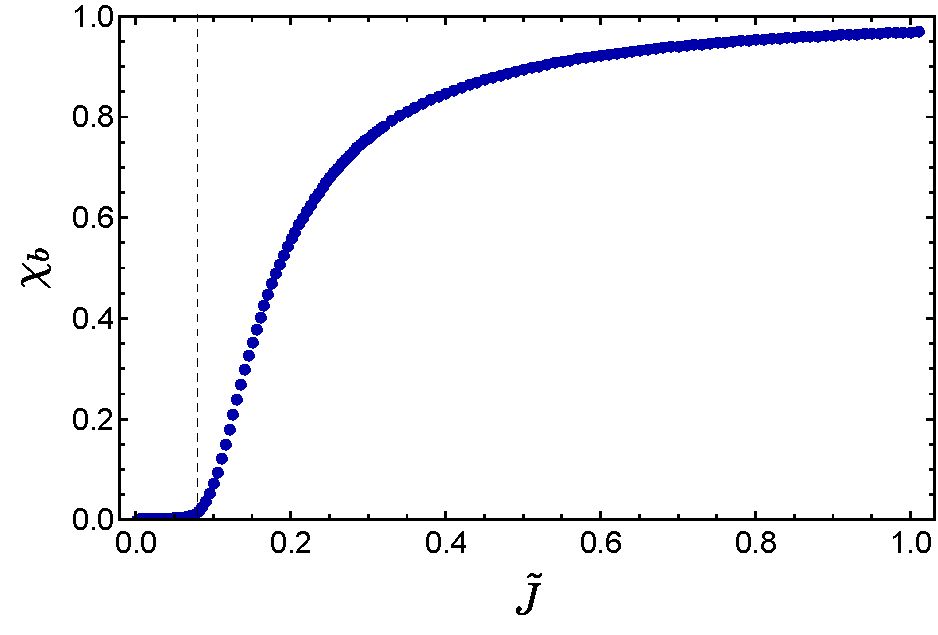
\includegraphics[width= .7\textwidth]{images/CH4/b.pdf}
    \caption{Mean-field parameter $\chi_b$ versus $\tilde{J}$. Dashed line indicates $\tilde{J}_c$.}
    \label{fig:4-b}
\end{figure}
\begin{figure}[h]
    \centering
    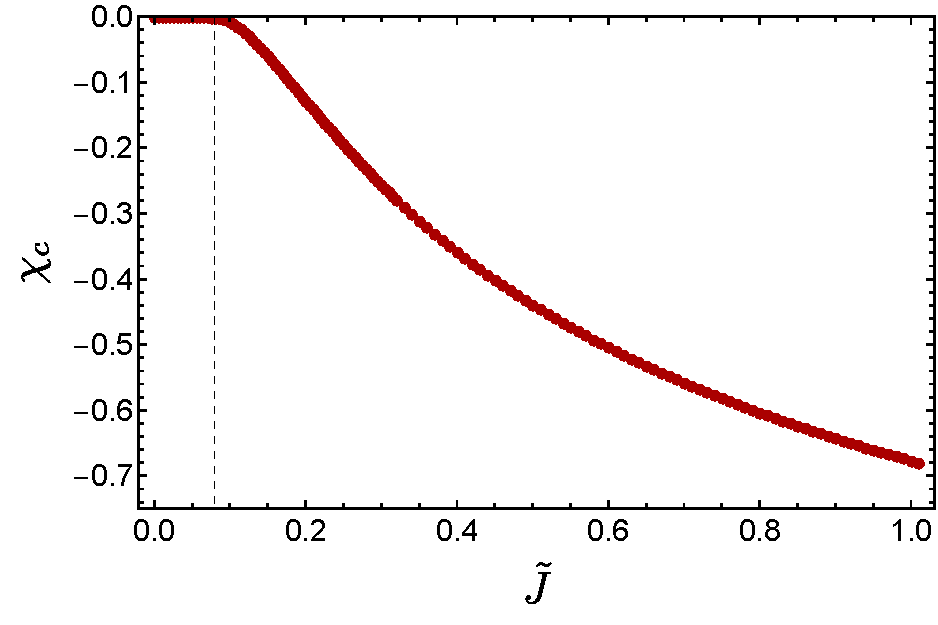
\includegraphics[width= .7\textwidth]{images/CH4/c.pdf}
    \caption{Mean-field parameter $\chi_c$ versus $\tilde{J}$.}
    \label{fig:4-c}
\end{figure}

%\begin{figure}[ht]
%    \centering
%    \begin{subfigure}{.5\textwidth}
%        \centering
%        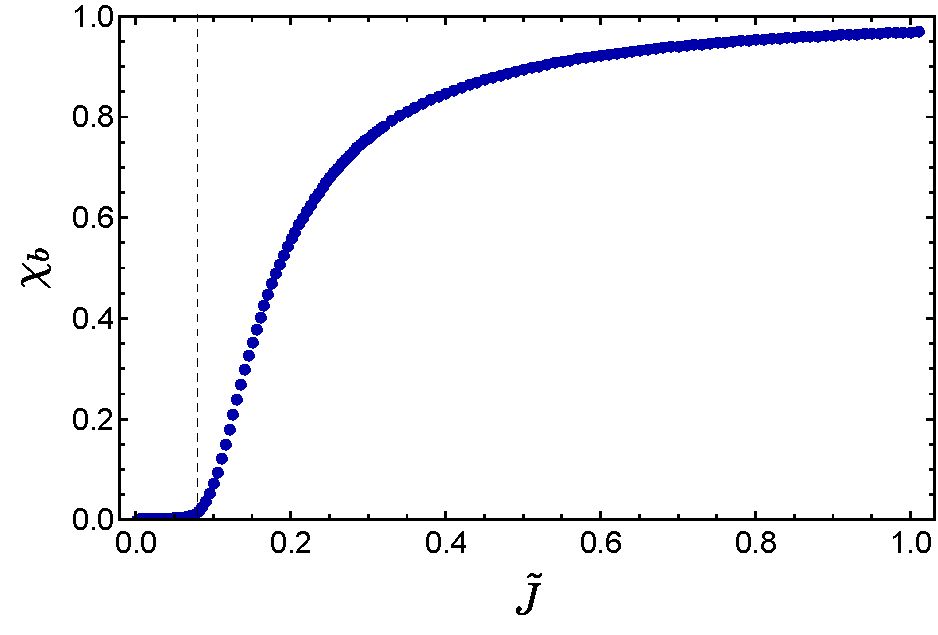
\includegraphics[width= \textwidth]{images/CH4/b.pdf}
%        \caption{mean-field parameter $\chi_b$ versus $\widetilde{J}$}
%        \label{fig:4-b}
%%    \begin{subfigure}{.5\textwidth}
% %       \centering
%        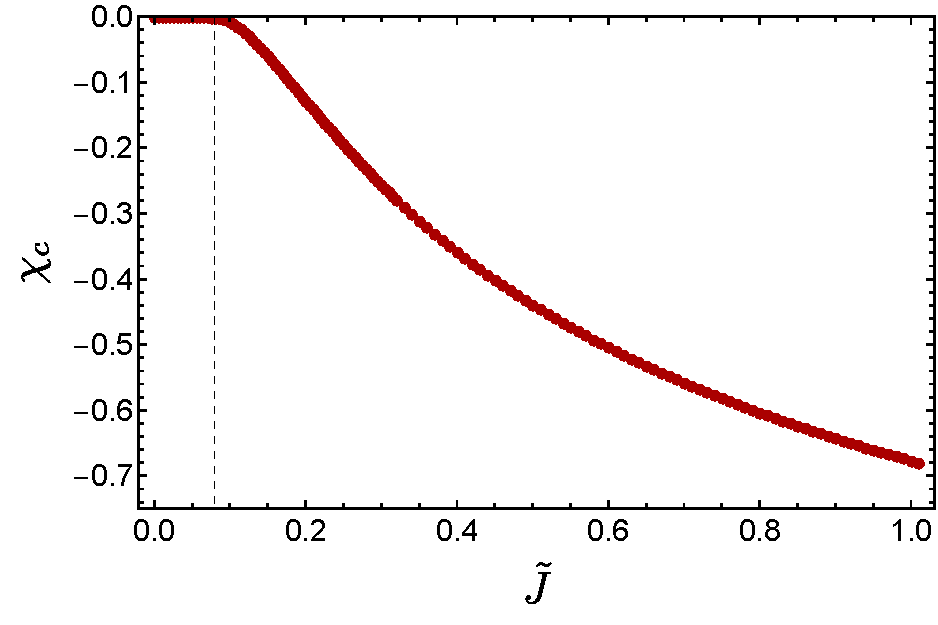
\includegraphics[width= \textwidth]{images/CH4/c.pdf}
%        \caption{mean-field parameter $\chi_c$ versus $\widetilde{J}$}
%        \label{fig:4-c}
%    \end{subfigure}
%\caption{ Numerical calculation of the Mean field phase diagram with $\bf{h} = 0.85 \, J \, \bf{c}$ . Also, the lattice linear dimensions are $\ell_x = \ell_y = 250$ and was find that $\tilde{J}_c = 0.08 \pm 0.01$. }%
%\end{figure}

The numerical calculation for the figures \ref{fig:4-b} and \ref{fig:4-c} was done for a magnetic field $\bf{h} = 0.85 \, J \, \bf{c}$, the lattice linear dimensions used were $\ell_x = \ell_y = 250$ and was find that $\tilde{J}_c = 0.08 \pm 0.01$. For different strength and directions of the field the value of $\tilde{J}_c$ changes, in particular it increase monotonically with the absolute vale of the magnetic field.


This result ratifies that the situation in which for sufficiently small interaction across the defect, $\tilde{J}<\tilde{J}_c$, the ground state will be in a uncoupled phase. In this situation, the are no coupling between the Majorana across the edges because $\chi_b=\chi_c=0$. This can also be seem in figure \ref{fig:4-MF-GL-disp}, in which the excitations are gapless in this regime. Thus, exist Majorana edge modes at the defect.

In the case of sufficiently strong interaction across the defect, $\tilde{J}>\tilde{J}_c$, the Majoranas between the edges couples and the phase become gapped. This can be seem in figure \ref{fig:4-MF-GD-disp}. The excitations have a non-zero gap, $\Delta_{\gamma}$, in this phase.

In this uncoupled regime, the mean-field Hamiltonian \eqref{eq:4-MF-Ham} reduces to the theory explained in chapter \ref{ch:3}.


\begin{figure}[ht]
    \centering
    \begin{subfigure}{.49\textwidth}
        \centering
        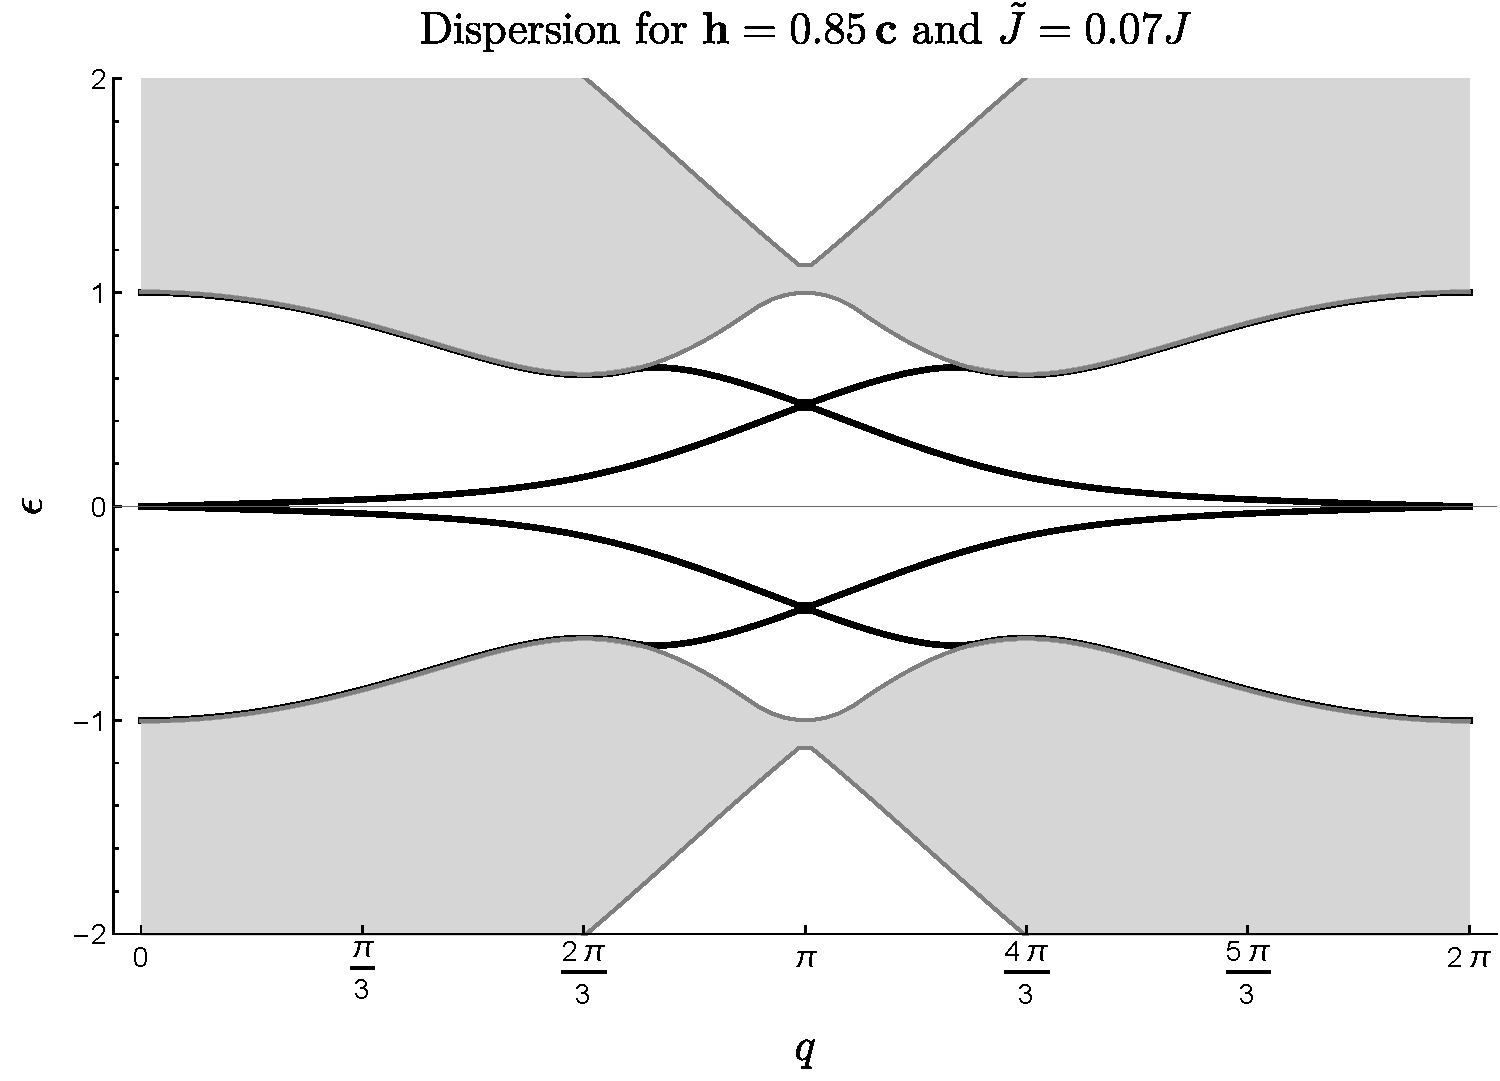
\includegraphics[width= \textwidth]{images/CH4/disp_MF_Gapless.pdf}
        \caption{Dispersion for  $\tilde{J}< \tilde{J}_c$.}
        \label{fig:4-MF-GL-disp}
    \end{subfigure}\hspace{1mm}%
    \begin{subfigure}{.49\textwidth}
        \centering
        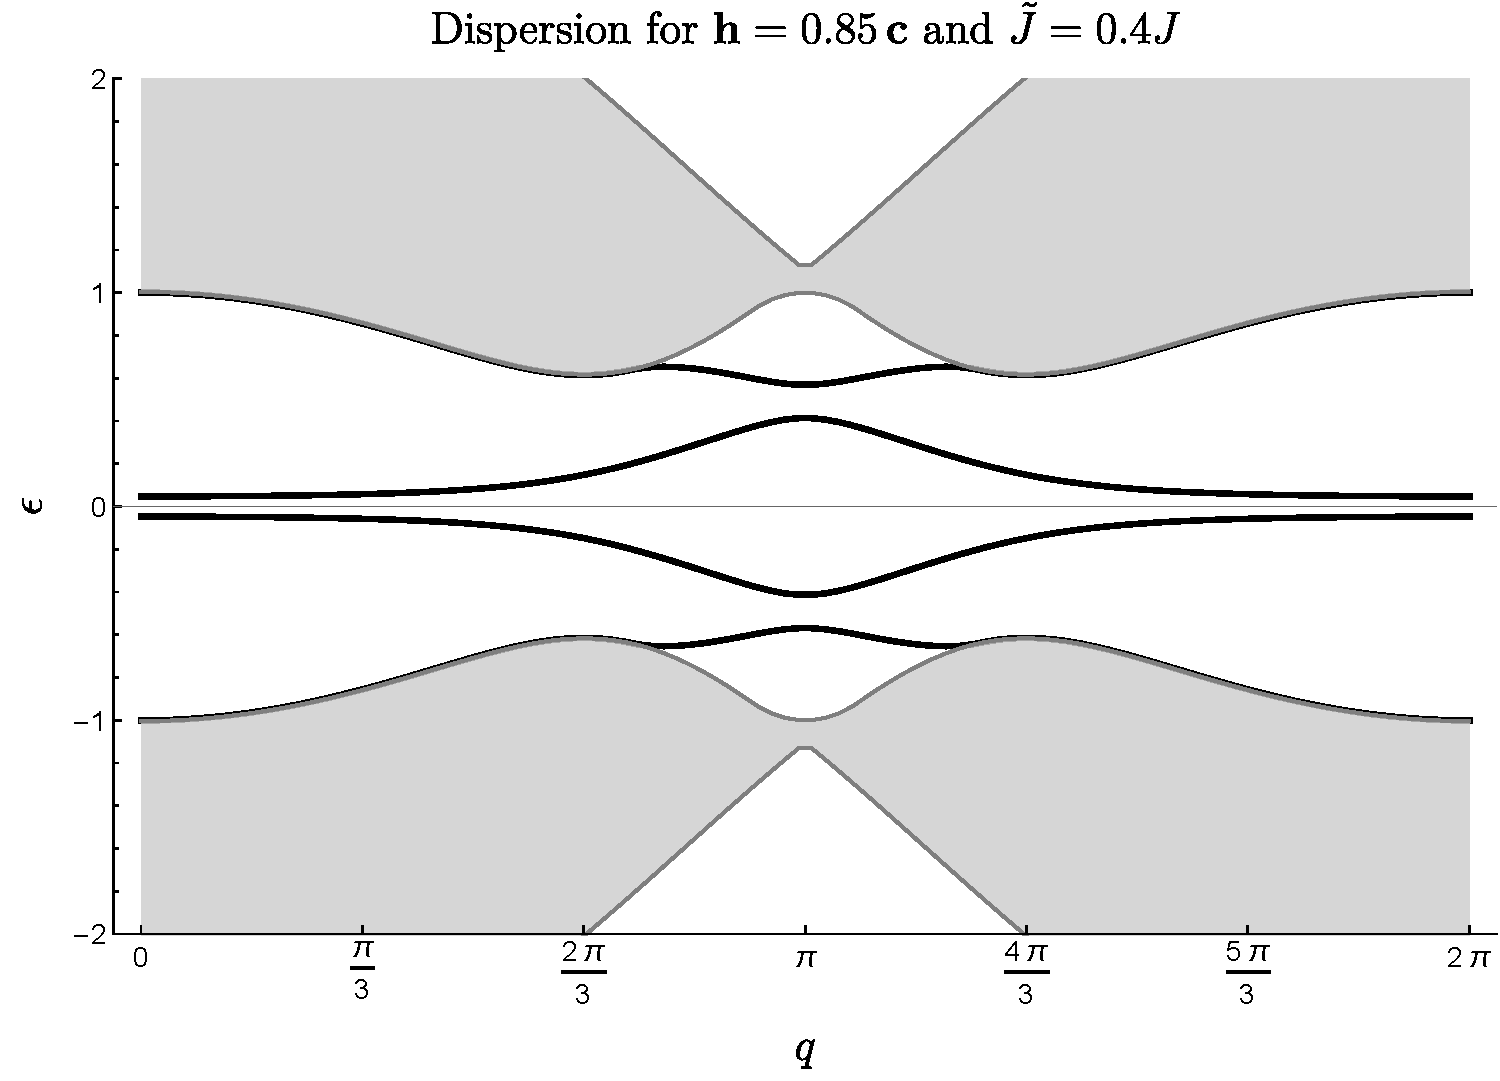
\includegraphics[width= \textwidth]{images/CH4/disp_MF_Gapped.pdf}
        \caption{Dispersion for  $\tilde{J} > \tilde{J}_c$.}
        \label{fig:4-MF-GD-disp}
    \end{subfigure}
\caption{ Dispersion numerically calculated using the mean-field approximation. For weak interaction between the edges \ref{fig:4-MF-GL-disp}, the dispersion is indistinguishable form the dispersion without the interaction \ref{fig:3-disp-c}. For strong interaction \ref{fig:4-MF-GD-disp}, the modes localized in the edge acquires a gap.    }
\end{figure}




The mean-field calculation is useful to identify the existence of the two phases described before. %As for predict the exact value of $\tilde{J}_c$ the mean-field approximation is not good. For example, even under the mean field approximation I believe that the phase transition occurs is a slight greater than the predicted value. For example, in figure \ref{fig:4-MF-disp-critical} it shown that the Majorana modes remains uncoupled even for values slight higher than predicts in the first calculation using the mean-field approximation.
However, the mean-field analysis is not enough to determine the precise location of the phase transition. 


Complementary to the analysis from the mean-field parameters, the energy gap for the Majorana edge modes describes if these modes are coupled or not. Interestingly, even beyond the critical point predicted from the mean-field analysis the gap remains rather small. For practical purposes, the system behaves as in the uncoupled phase when this gap is smaller than the energy scale set by temperature. In the figure \ref{fig:4-gap} is shown the magnitude of the gap in function of the coupling.
%\begin{figure}[h]    \centering    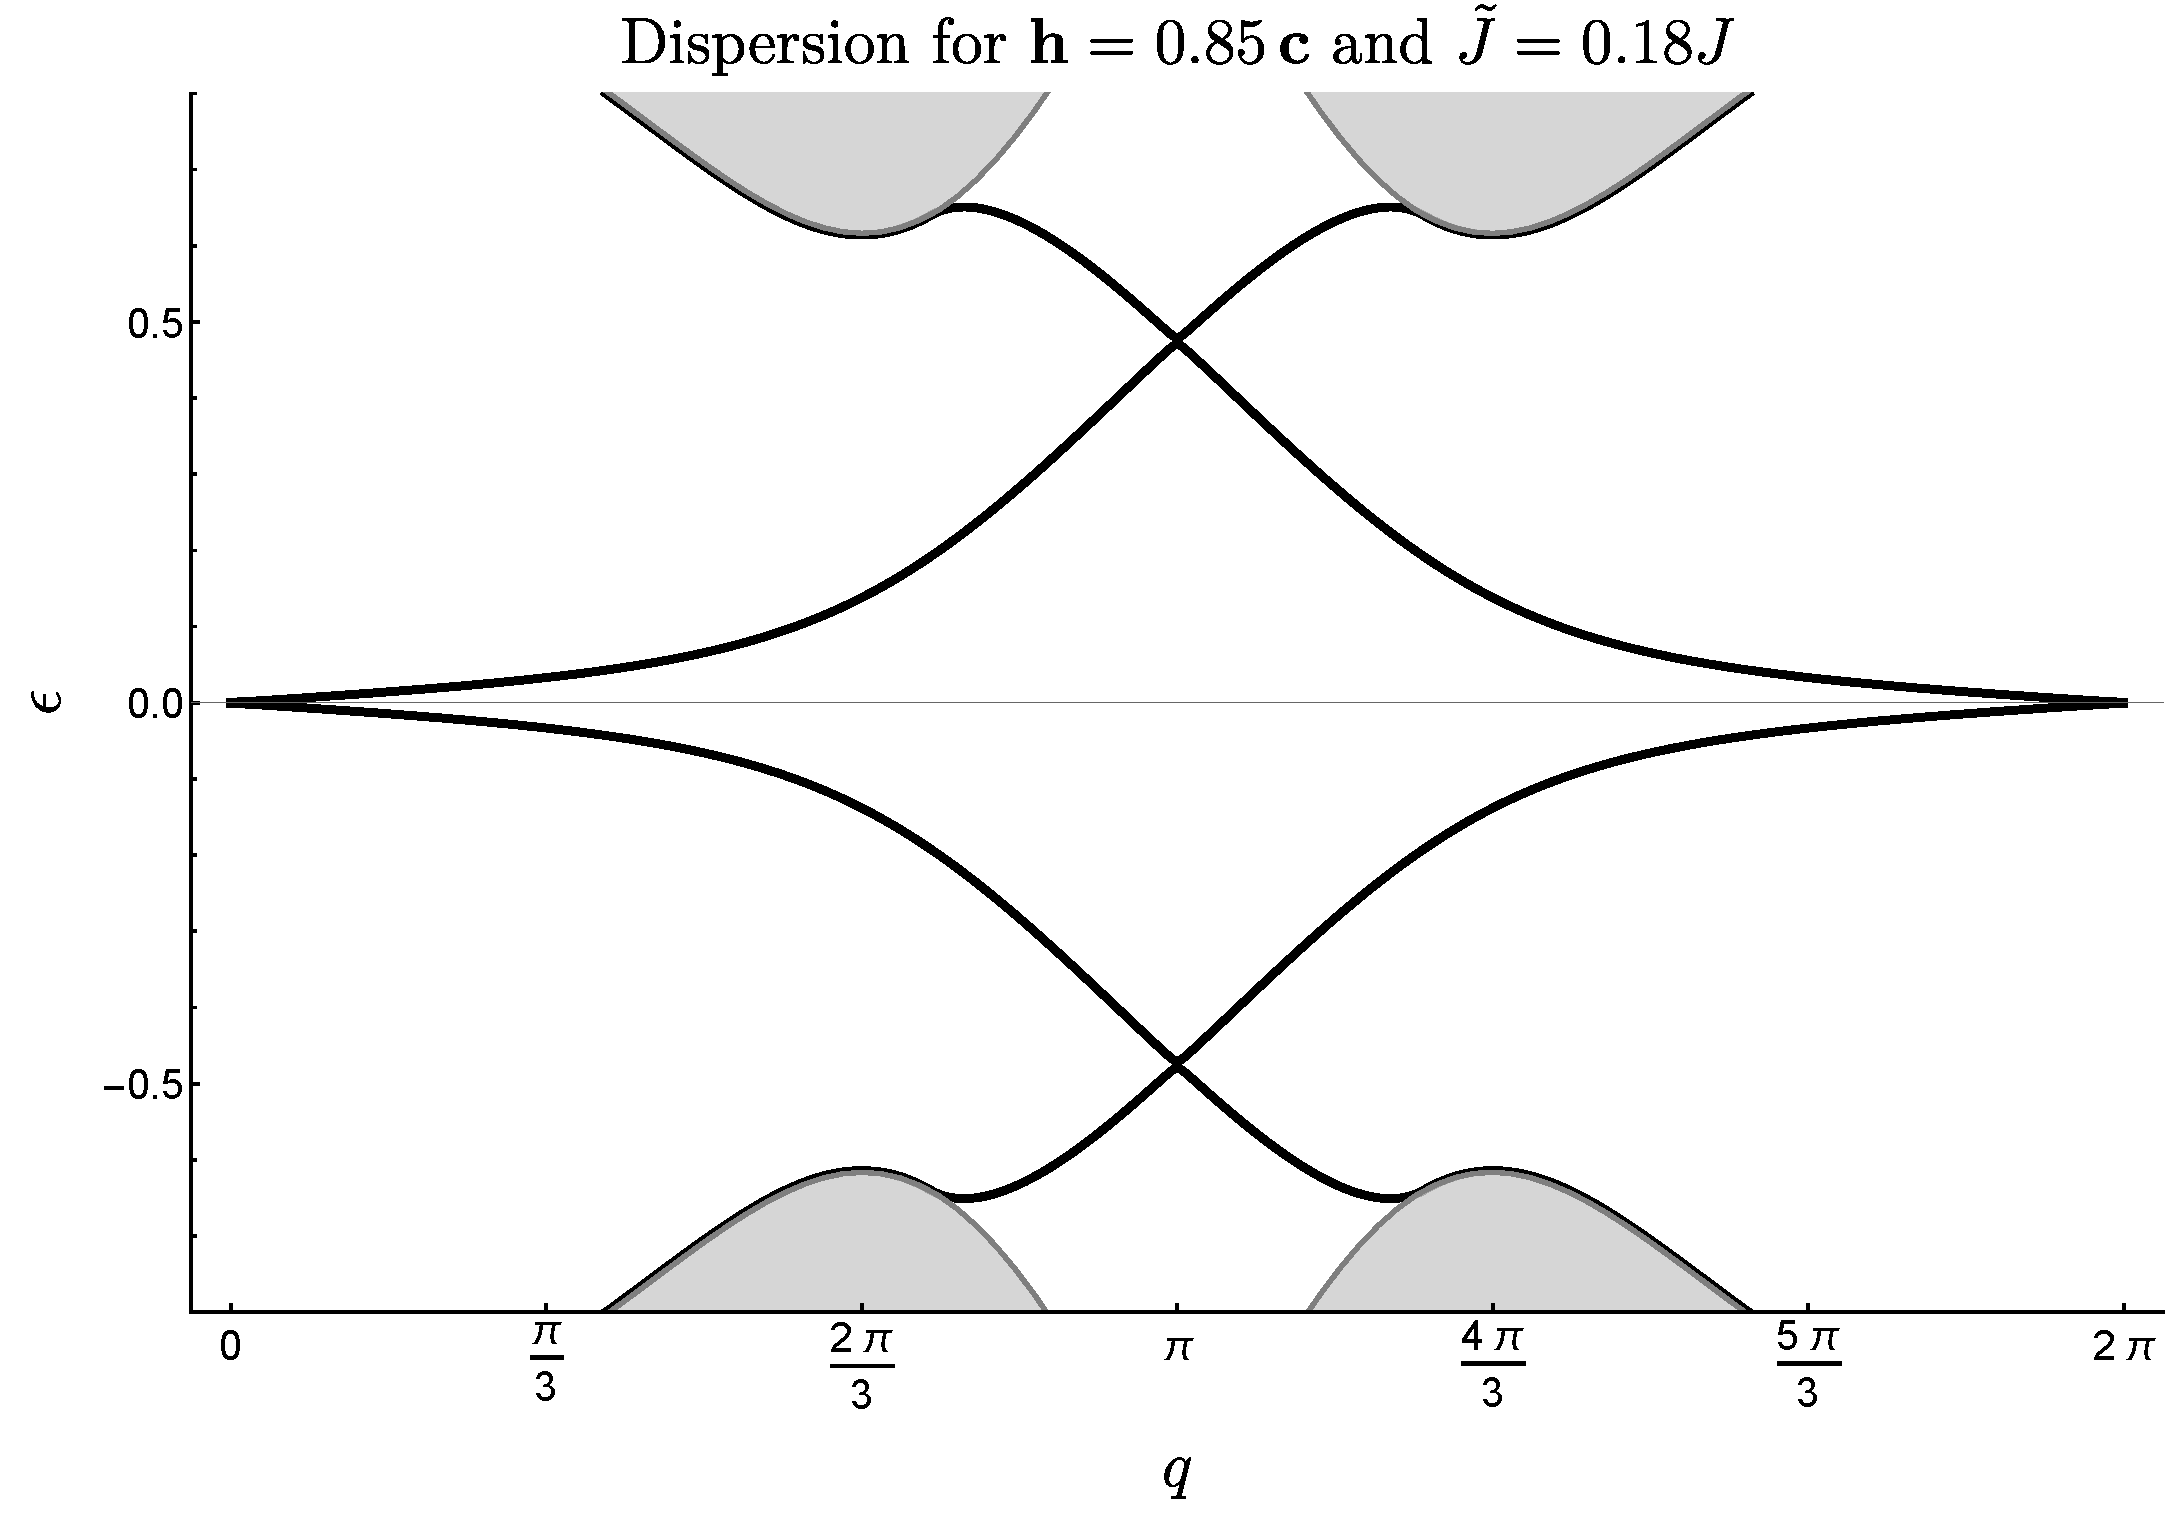
\includegraphics[width= .51\textwidth]{images/CH4/disp-zoom-critical18.pdf}    \caption{Dispersion using the mean-field approximation for $\widetilde{J} \gtrapprox \tilde{J}_c$.  }    \label{fig:4-MF-disp-critical}\end{figure}

\begin{comment}

\end{}
\begin{figure}[t]
    \centering
    \begin{subfigure}{.49\textwidth}
       \hspace*{-5mm}
        \centering
        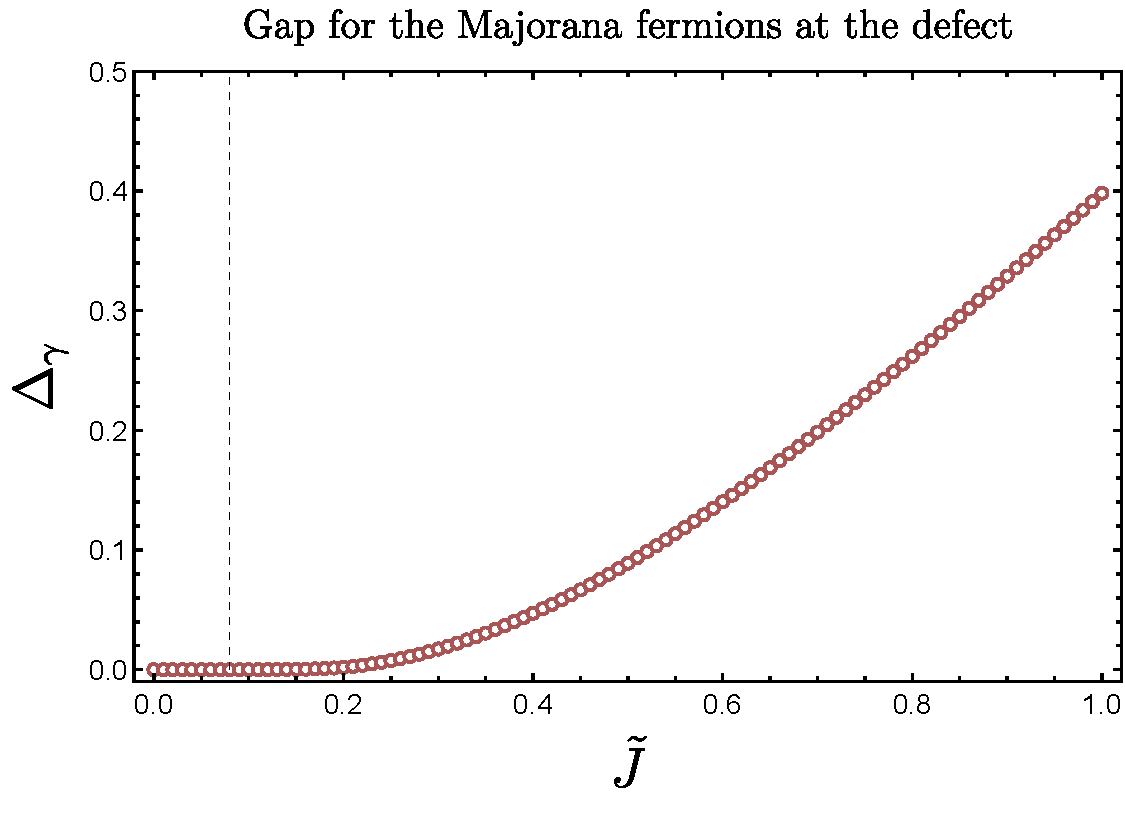
\includegraphics[width=.95\textwidth]{images/CH4/gap_no_fit.pdf}
        \caption{Energy gap as function of $\tilde{J}$.}
        \label{fig:4-gap}
    \end{subfigure}\hspace{1mm}%
    \begin{subfigure}{.49\textwidth}
        \centering
         \hspace*{-5mm}
        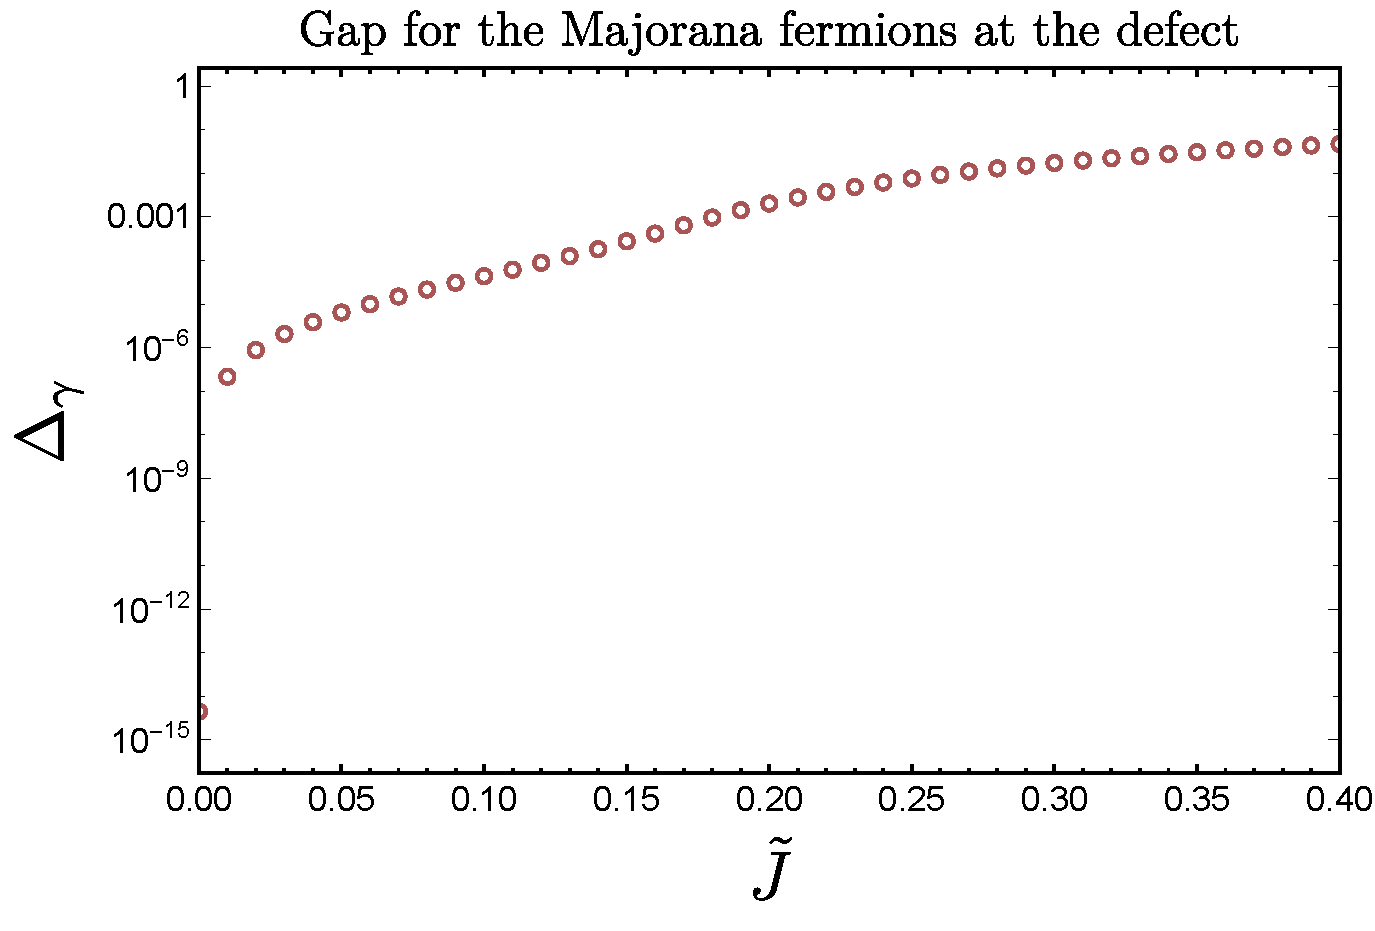
\includegraphics[width=.95\textwidth]{images/CH4/gap_Log_no_fit.pdf}
       % \hspace{5mm}
        \caption{Log-linear inspection of figure \ref{fig:4-gap}.}
        \label{fig:4-Log-gap}
    \end{subfigure}
\caption{ Energy gap increases with the coupling $\tilde{J}$.}
\end{figure}
\end{comment}

\begin{figure}
    \centering
    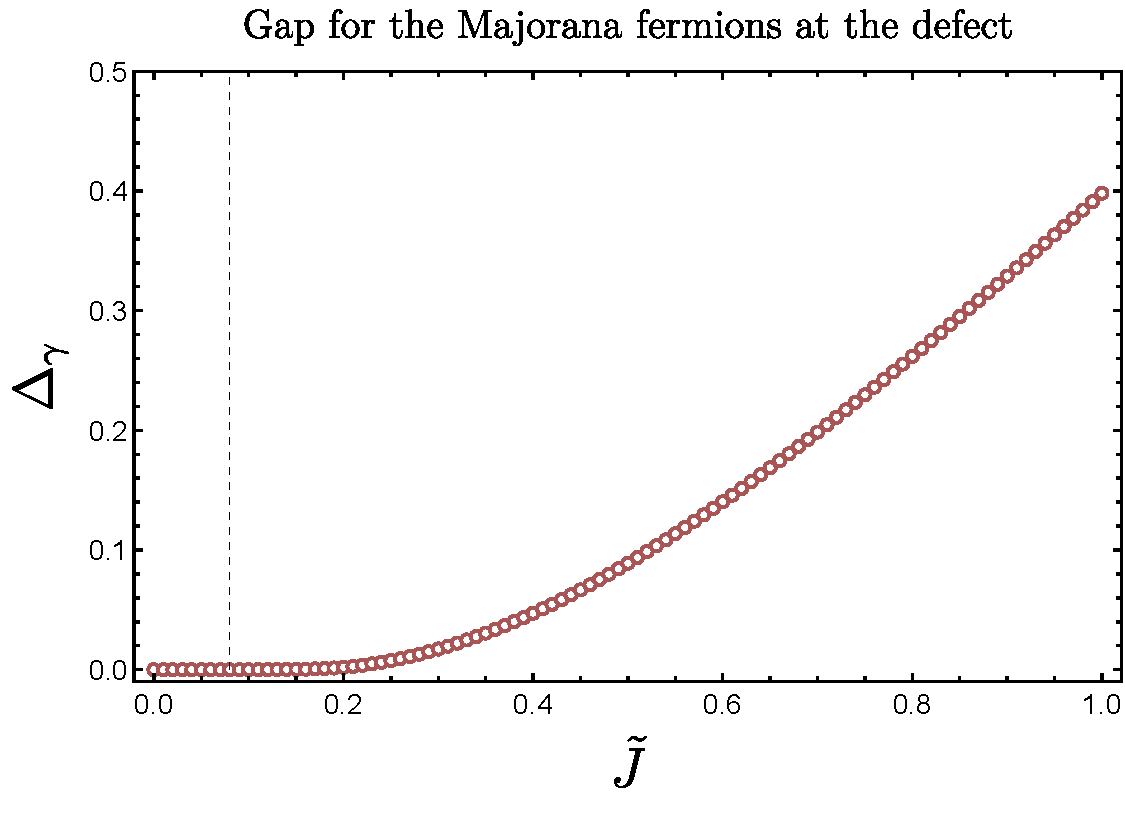
\includegraphics[width=.6\textwidth]{images/CH4/gap_no_fit.pdf}
        \caption{Energy gap for Majorana fermions in the defect as function of $\tilde{J}$.}
        \label{fig:4-gap}
\end{figure}


In this chapter we have seen that there is a phase in which the Majorana modes in the defects remain gapless and uncoupled. With respect to the significance of this result, it should be noted that even small separation between the atoms can drastically decrease the coupling constant, see Ref.\cite{Yadav_2018}. Thus, I expect the coupling $\tilde{J}$ in defects to be sufficiently small to host uncoupled gapless Majorana fermions.

In the next chapter, I will work out the low-energy effective theory for the defect-bound Majorana modes that remain gapless in this weakly interacting regime.












